% Suggested topics:
% Maybe something about what makes CDT different from DT, how causality is implemented?

\begin{frame}
    \frametitle{Goal}
    Extract information from Quantum Gravity path integral:
    \begin{equation}
        Z = \int \mathcal{D}[g_{\mu \nu}] e^{i S[g_{\mu \nu}]}
    \end{equation}
    With Einstein-Hilbert action:
    \begin{equation}
        S[g_{\mu \nu}]
        =
        \frac{1}{16 \pi G}
        \int_\mathcal{M} \dd[4]{x} \sqrt{-g}
        (R(x) - 2 \Lambda)
    \end{equation}
    Problem: How can we integrate over geometries? \\
    Solution: Triangulations!
\end{frame}

\begin{frame}
    \frametitle{Causal Dynamical Triangulations}
    \begin{columns}
        \begin{column}{0.7\textwidth}
            Create causal structure:
            \begin{itemize}
                \item In (1 + 1)D: use triangles
                \item Timeslice: ring of $L$ links
                \item Universe: sequence of $T$ timeslices connected by triangles
            \end{itemize}
            Example: $T = 3$, $L = 5$, $N = 2TL = 30$
        \end{column}
        \begin{column}{0.3\textwidth}
            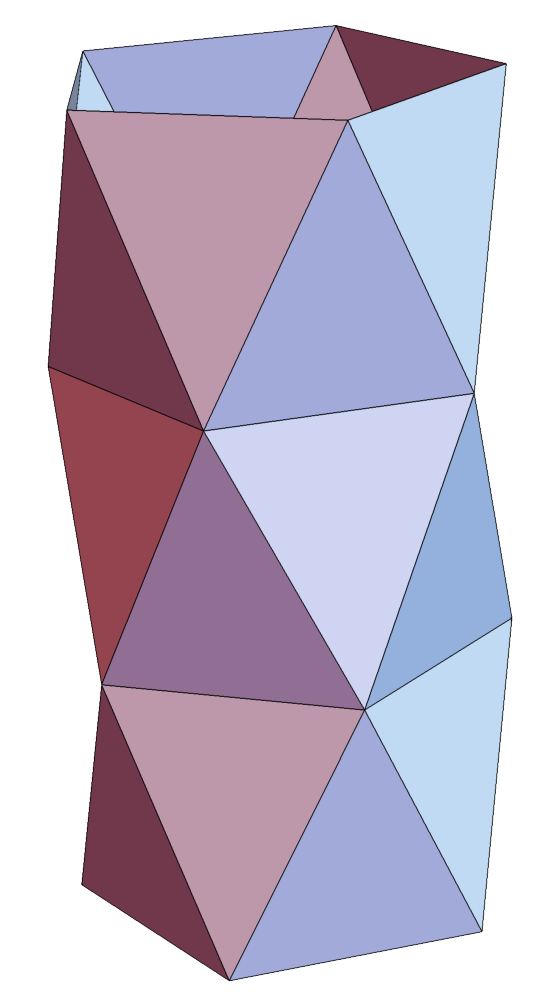
\includegraphics[width=1\textwidth]{uniform}
        \end{column}
    \end{columns}
\end{frame}

\begin{frame}
    \frametitle{Technicalities}
    Some technicalities:
    \begin{itemize}
        \item In 2D: constant curvature
        \item Action proportional to volume ($N_2$)
        \item Wick rotation
        \item Label triangles
    \end{itemize}
    Resulting partition function:
    \begin{equation}
        Z_\ell = \sum _{T_\ell} \frac{1}{N_2(T_\ell)!} e^{-\lambda N_2(T)}
    \end{equation}
\end{frame}